\newpage
\section{Alberi decisionali}
Prendiamo ora un esempio di training set di partite di tennis e costruiamo l'albero decisionale.
\begin{figure}[h!]
    \centering
    \begin{subfigure}{.45\textwidth}
        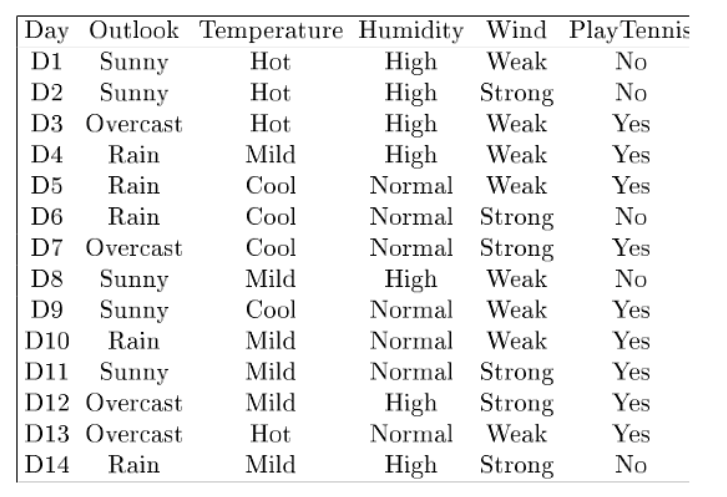
\includegraphics[width=\textwidth]{images/tennis-training-set.png}
    \end{subfigure}
    \begin{subfigure}{.45\textwidth}
        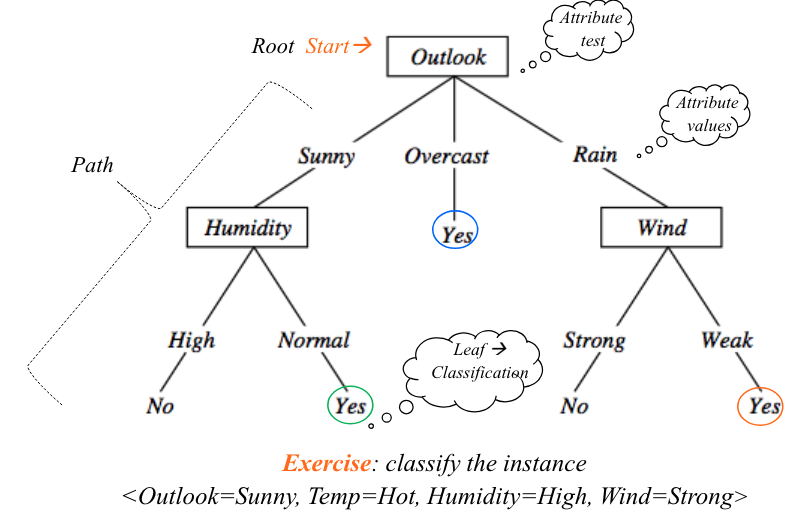
\includegraphics[width=\textwidth]{images/decision-tree-tennis.png}
    \end{subfigure} 
\end{figure}

\hspace{-15pt}Un albero decisionale rappresenta una disgiunzione di congiunzioni di vincoli sul valore
degli attributi.
\begin{enumerate}
    \item (verde) (Outlook = Sunny $\land$ Humidity = Normal) $\land$
    \item (blu) (Outlook = Overcast) $\land$
    \item (rosso) (Outlook = Rain $\land$ Wind = Weak)
\end{enumerate}
H di DT capace di esprimere qualsiasi funzione finita a valori discreti (proposizionale).

\subsection{ID3 algorithm}
ID3 è un algoritmo base per l'apprendimento sui decision tree. Dato un training set di esempi, l'algoritmo per costruire
un decision tree esegue una ricerca nello spazio dei decision tree. La costruzione dell'albero è di tipo \textbf{top-down} e l'algoritmo
esegue una ricerca di tipo \textbf{greedy}.\\\\
La domanda fondamentale è "quale attributo dovrebbe essere testato successivamente? Quale domanda ci dà più informazioni"
\begin{itemize}
    \item Selezionare il \textbf{miglior attributo}
    \item Viene quindi creato un nodo discendete per ogni possibile valore di questo attributo e gli esempi sono suddivisi in base a questo valore.
    \item Il processo viene ripetuto per ogni nodo successore finché tutti gli esempi sono classificati correttamente o non ci sono più attributi.
\end{itemize}
\begin{lstlisting}
    // X: esempi di training
    // T: attributo target
    // Attrs: altri attributi, inizialmente tutti gli attributi
    ID3(X, T, Atter) 
        Create Root Node
        if all X are +: return Root with class +
        if all X are -: return Root with class -
        if Attrs is empty: return Root with class most comon value of T in X
        else 
            A <- best attribute; decision attribute for Root <- A
            for each possible value v_i of A:
                add a new branch bellow Root, for test A = v_i
                X_i <- subset of X con A = v_i
                if X_i is empty then 
                    add a new leaf with class the most common value of T in X
                else then
                    add the subtree generated by ID3(X_i, T, Attr - {A})
        return Root
\end{lstlisting}
Andiamo ad usare la nozione di \textbf{entropia}, comunemente usata nalla teoria dell'informazione.
L'entropia misura l'impurità di una collezione di esempi. Essa dipende dalla distribuzione di una variabile randomica $p$
\begin{itemize}
    \item $S$ è una collezione di esempi di trining.
    \item $p_+$ la proporzioni di esempi positivi in $S$.
    \item $p_-$ la proporzione di esempi negativi in $S$.
\end{itemize}
\begin{definition}
    Definiamo matematicamente \textbf{entropia} come:
    $$Entropy(S) \equiv -p_+ \log_2 p_+ - p_- \log_2p_- \hspace{15pt} [assumento \:\: 0\log_2 0 = 0]$$
\end{definition}
\begin{example}
    Alcuni esempi possono essere i seguenti:
    \begin{itemize}
        \item $Entropy([14+, 0-]) = -14/14\log_2(14/14) - 0\log_2(0) = 0$
        \item $Entropy([9+, 5-]) = -9/14\log_2(9/14) - 5/14\log_2(5/14) = 0.94$
        \item $Entropy([7+, 7-]) = -7/14\log_2(7/14) - 7/14\log_2(7/14) = 1/2 + 1/2 = 1$ questo è un caso con alta inpurità
    \end{itemize}
\end{example}
\begin{note}
    Notare che $0 \leq p \leq 1, 0 \leq entropy \leq 1$
\end{note}
\begin{figure}[h!]
    \centering
    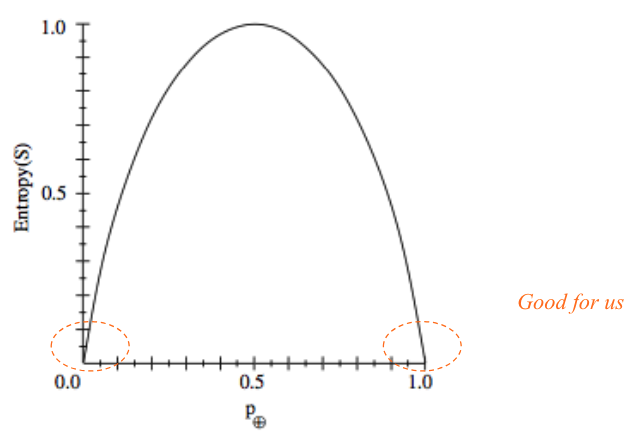
\includegraphics[width=0.5\textwidth]{images/entropia.png}
\end{figure}
Se abbiamo tutti i +1 o tutti i -1 allora abbiamo 0 entropia cioè "no informazioni". Il massimo per $S$ la abbiamo invece con esempi 1/2+ e 1/2-.\\\\
Il guadagno di informazioni è la riduzione prevista dell'entropia causata partizionando gli esempi su un attributo. 
\begin{definition}
    Definiamo la \textbf{Riduzione attesa dell’entropia conoscendo A}
    $$Gain(S, A) = Entrpy(S) - \sum_{v \in Values(A)}\frac{|Sv|}{|S|}Entropy(Sv)$$
    Dove $values(A)$ sono i possibili valori per A, mentre $Sv$ è un sottoinsieme di esempi di S per i quali A ha valore v (somma di pesi)
\end{definition}
\hspace{-15pt}Maggiore è il guadagno di informazione, più efficace è l'attributo classificazione dei dati di addrestramento (maggiore variazione nell'omogeneità dei distribuzione delle classi nei sottoinsiemi, massima separazione delle classi).
\textbf{Omogeneo}, poiché [14+, 0-] o [0+,7-] ci consentono una classificazione “chiara”.\\\\
L'entropia misura l'omogeneità (anzi impurità) della classe del sottoinsieme di esempi, quindi: \textbf{Selezionare A che massimizzi}
$$Gain(S, A) = Entropy(S) - \sum_{v \in Values(A)} \frac{|Sv|}{|S|} Entropy(Sv)$$
Dopo la suddivisione, valori più bassi (obiettivi più omogenei) in ciascun sottoinsieme porta ad un guadagno più elevato.
Lo scopo è quello di separare gli esempi in base al target, trovare l'attributo che discimina gli esempi a cui appartengono diverse classi target.
\begin{figure}[h!]
    \centering
    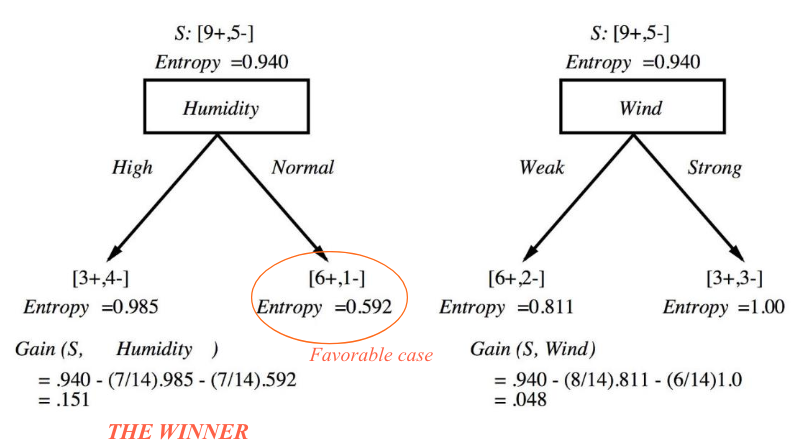
\includegraphics[width=0.6\textwidth]{images/esempio-select-best-attribute.png}
\end{figure}
\\
\begin{minipage}{0.65\linewidth}
    Il guadagno di informazioni favorisce attributi con molti valori possibili. Consideriamo l'attributo "Date" nell'esempio "PlayTennis".\\\\
    "Date" ha il massimo guadagno di informazioni. Ogni giorno corrisponde ad un sottoinsieme differente che è puro: $[1+, 0-]$ o $[0+, 1-] \to 0$ entropia. 
    Abbiamo un adattamento perfetto (separazione) dei dati di trining, ma non è significato: non serve per i casi invisibili. \\\\
    Chiediamoci ora come evitare la generazione di molti piccoli
    sottoinsiemi?    
\end{minipage}
\hfill
\begin{minipage}{0.35\linewidth}
    \centering
    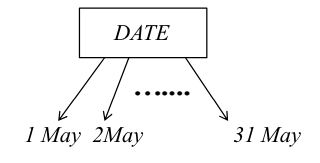
\includegraphics[width=0.95\textwidth]{images/problem-information-gain.png}
\end{minipage}
\begin{definition}
    Definiamo quello che è chiamato \textbf{gain ratio}
    $$GainRation(S, A) = \frac{Gain(S, A)}{SplitInInformation(S, A)}$$
    Dove abbiamo che:
    $$SplitInInformation(S, A) = -\sum_{i=1}^{C}\frac{|S_i|}{|S|} \log_2\frac{|S_i|}{|S|}$$
\end{definition}
\hspace{-15pt}Abbiamo che $S_1$ sono degli insiemi ottenuti partizionando sul valore $v_i$ di $A$ finao al valore $c$.
SplitInInformation misura l'entropia di S rispetto ai valori di A, Più i dati sono distribuiti uniformamente, più sono alti.\\\\
Il GainRation penalizza gli attributi che dividono gli esempi in molte piccole classi come per Date.
Sia $|S| = n$ la divisione degli esempi di date in $n$ sottoinsiemi.
$$SplitInInformation(S, Date) = -[(1/n \:\log_2 1/n)) + \dots + (1/2 \log_2 1/n)] = -\log_2 1/n = \log_2n$$
Il quale è $> 1$ per $n > 2$ quindi riduciamo il GainRatio.\\
Confronto con un A che divide i dati in due classi pari (con $(n/2)/n = 1/2$):
$$SplitInInformation(S, A) = -[(1/2 \log_2 1/2) + (1/2\log_2 1/2)] = -[-1/2 - 1/2] = 1 \to \text{ no reduction }$$
Abbiamo un problema: $SplitInInformation(S, A)$ può essere zero o molto piccolo quando $|S_i|\approx |S|$ per qualche valore $i \: [\log 1 = 0]$.
Per mitigare questo effetto, vengono usate le seguenti euristiche:
\begin{enumerate}
    \item Calcolare $Gain$ per ogni attributo.
    \item Applicare $GainRation$ solo per gli attributi con $Gain$ sopra la media.
\end{enumerate} 
La ricerca nello spazio delle ipotesi attraverso ID3 consiste nel cercare (hill-climbing) attraverso lo spazio delle possibili
DT dal più semplice al sempre più complesso. W.r.t. per l'algoritmo precedente:
\begin{minipage}{.6\linewidth}
    \begin{itemize}
        \item Lo spazio delle ipotesi è completo (rappresenta tutti i valori discreti funzioni).
        \item Nessun passo indietro; nessuna garanzia di ottimalità (ottimale locale).
        \item Utilizza tutti gli esempi disponibili (non incrementale)
        \item Può terminare prima, accettando classi "rumorose"
    \end{itemize}
\end{minipage}
\hfill
\begin{minipage}{.4\linewidth}
    \centering
    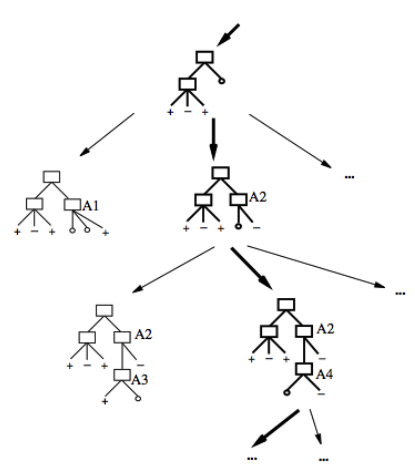
\includegraphics[width=0.8\textwidth]{images/hp-space-search-dt-learning.png}
\end{minipage}
Parliamo ora degli \textbf{bias induttivi} nell'apprendimento per i decision-tree. Quali sono?
\begin{enumerate}
    \item Gli alberi più piccoli sono preferibili rispetto a quelli più grossi. A causa della ricerca da semplice a complessa, incrementalmente.
    Questo però non è sufficiente questo sarebbe il bias che esibirebbe un semplice algoritmo beadth first generando tutti i DT e selezionando quello più breve e coerente.
    \item Preferiamo alberi che posizionano l'informazion gain più alto pià vicina alla root.
\end{enumerate}
\begin{note}
    DT non sono limitare alla rappresentazione tutte le possibili funzioni, la restizione non riguarda lo spazio delle ipotesi, ma la strategia di ricerca.
\end{note}
\begin{definition}
    Definiamo le preferenze o \textbf{search biad} (dovute alla strategia di ricerca). \\\\
    ID3 ricerca uno spazio completo di ipotesi, la strategia di ricerca è incompleta.
\end{definition}
\begin{definition}
    Definiamo le restrizione o \textbf{language bias} (a causa dell'insieme di ipotesi esprimibile o consideto).\\\\
    Visto nel candidate-elimination dove sono ricercati in uno spazio di ipotesi incompleto, la strategia di ricerca è completa (tutte le ipotesi consistenti, nel version space)
\end{definition}
Perché il search bias viene preferito rispetto al language bias? Nel ML tipicamente si usano aprocci \textbf{flessibili} (capacità universale dei modelli) senza
escludere a priori la funzione bersaglio sconosciuta. Ovviamente la flessibilità può portare a problemi di overfitting.\\\\
Perché preferire ipotesi più brevi? Come disse Ockham nel 1300 con il razoio di Occam "La spiegaione più semplice è più probabilmente quella corrette" o
"Prefrisco l'ipotesi più semplice che si adatta ai dati" Il termine rasoio si riferisce all'atto di radere via inutili ipotesi per arrivare alla spiegazione più semplice. Viene anche detta
"Legge di parsimonia" o "legge di economia".\\\\
Ricorda il "controllo della complessità del modello" mediante la regolarizzazione per modelli lineari. Ancora, questo concetto fondmanetale
nel ML verrà ritrovato e "razzionalizzato" più avanti.

\subsection{Risolvere problemi ID3}
Ci sono diverse problematiche nell'apprendimento per gli alberi di decisioni fra questi abbiamo:
\begin{itemize}
    \item Overfitting. Che si divide a sua volta in: arresto anticipato, ridotta potature degli errori, regola post-potatura.
    \item Estensioni (specifico per i DT): attributi a valore contino, gestire esempi di formazione con valori di attributo mancanti, gestire attributi con costi diversi, miglioramento dell'efficienza computazionle.
\end{itemize}

\subsubsection{Overfitting}
Partiamo dal problema dell'overfitting. Costruire alberi che "si adattano troppo" agli esempi formativi può portare a un "overfitting". 
Consideriamo l'errore su un ipotesi $h$ su: dati di training: $error_D(h)$, intera distribuzione $X$ di dati: $error_X(h)$
\begin{definition}
    Si dice che l'ipotesi $h$ overfits i dati di trining se c'è un ipotesi alternativa $h' \in H$ tale che:
    $$error_D(h) < error_D(h') \hspace{10pt}e\hspace{10pt} error_X(h') < error_X(h)$$
    Cioè $h'$ si comporta peggio con i dati TR, meglio con i dati invisibili.
\end{definition}
\hspace{-15pt}Gli approcci flessibili possono facilmente incontrare un overfitting (se utilizzati senza cura speciale)
\begin{figure}[h!]
    \centering
    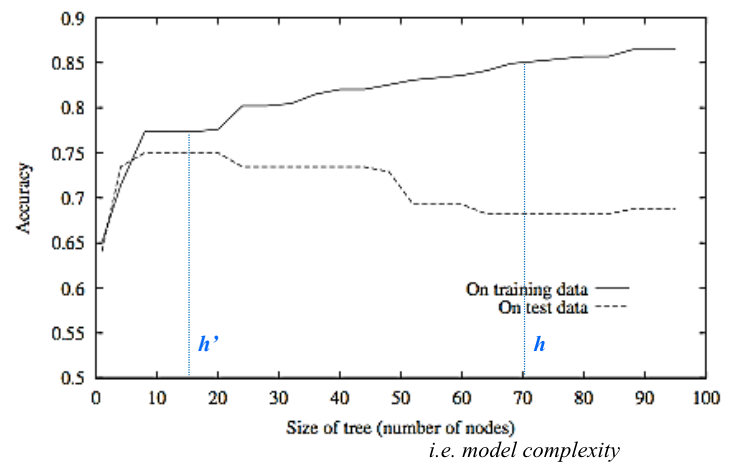
\includegraphics[width=0.6\textwidth]{images/overfitting-in-DT.png}
\end{figure}
\begin{example}
    Vediamo un esempio con dati "noisy".
    \begin{figure}[h!]
        \centering
        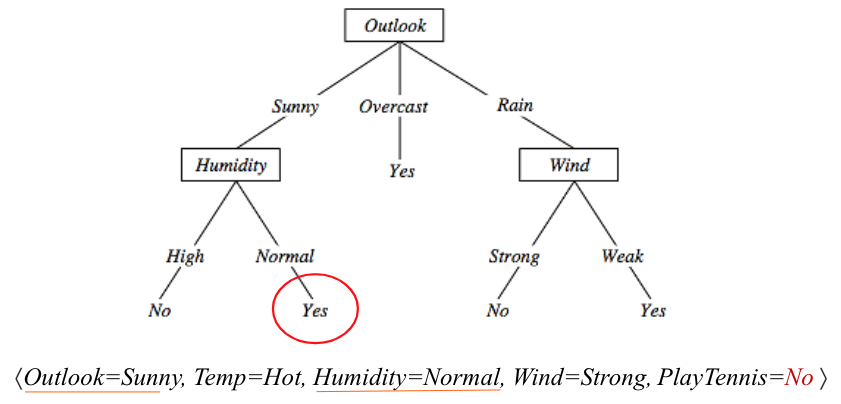
\includegraphics[width=0.6\textwidth]{images/example-noisy-data.png}
    \end{figure}

    \hspace{-15pt}Immagina che questo nuovo esempio rumoroso causi la divisione del secondo nodo foglia, allora DT cresce (la sua complessità cresce).
    Adattandosi anche al rumore, il nuovo DT è perfetto per i dati TR, non per i nuovi dati.
\end{example}
\hspace{-15pt}Per "evitare" l'overfitting nei DT, possiamo usare una di queste due strategie:
\begin{itemize}
    \item Smettere di far crescere l'albero prima, prima della classificazione perfetta ("arresto anticipato" vedere la trama prima)
    \item Consentire all'albero di adattarsi eccessivamente ai dati, quindi potare l'albero.
\end{itemize}
Come possiamo valutare l'effetto? Un primo modo può essere quello di usare un set di training e validazione, andando a divifere il training set
in due parti (training set e validation set) e utilizzare il set di validazione per valutare l'utilità di 1 e 2.\\\\
Altri approcci possono essere utilizzare un test statistico per stimare l'effetto dell'espansione o della potatura. \textbf{Principio della lunghezza minima}:
utilizza una misura di complessità per codificare il DT e gli esempi (classificati erroneamente) e interrompe la crescita dell'albero quando questa dimensione di codifica è minima.

\subsubsection{Reduced-error pruning}
Ogni nodo è un candidato per la potatura, la potatura consiste nel rimuovere un sottoalbero radicato in un nodo: il nodo diventa una foglia e gli
viene assegnata la classificazione più comune, i nodi vengono rimossi solo se l'albero risultate non ha prestazioni peggiori. I nodi vengono potati iterativamente:
ad ogni iterazione il nodo di cui la rimozione aumenta maggiormente la precisione del set di convalida e viene ridotta. La potatura si interrompe quando nessuna potatura aumenta la precisione.
\begin{figure}[h!]
    \centering
    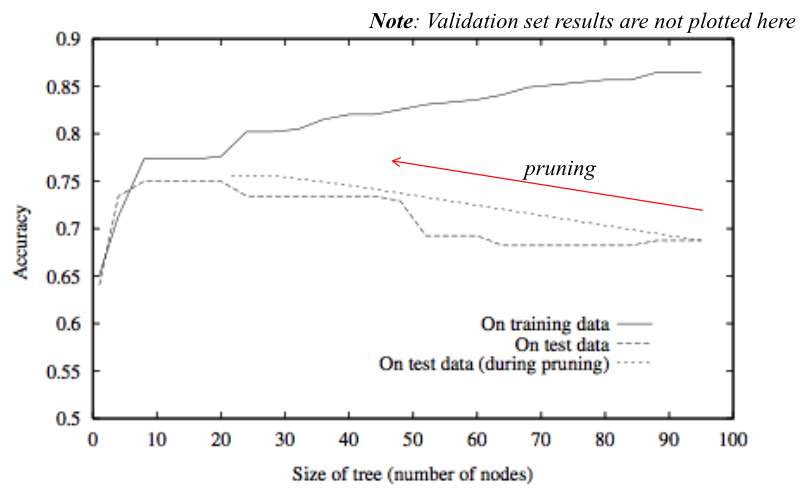
\includegraphics[width=0.6\textwidth]{images/effetto-reduced-error-pruning.png}
\end{figure}

\subsubsection{Regole post-potatura}
Abbiamo alcune regole che si applicano post-potatura:
\begin{enumerate}
    \item Create il decision tree dal training set.
    \item Convertire l'albero in un set di regole equivalente dove:
    \begin{itemize}
        \item Ogni \textbf{path} corrisponde ad una regola.
        \item Ogni \textbf{nodo} lungo un cammino corrispone ad una pre-condition.
        \item Ogni \textbf{foglia} classificata come post-condition.
    \end{itemize}
    Esempio: $(Outlook = Sunny) \land (Humidity = High) \land \Rightarrow (PlayTennis = No)$
    \item Potare (generalizza) ogni regola rimuovendo tali precondizioni la cui rimozione migliora la precisione oltre il set di validazione e oltre il training
    con una misura, statisticamente ispirata, pessimisitca.
    \item Ordina le regole in ordine di precisione stimato e considerale come una sequenza durante la classificazione di nuove istanze.
\end{enumerate}
Perché convertire in regole?\\
Ogni percorso distinto produce una regola diversa: una condizione di rimozione può basarsi su un criterio locale (contestuale),
l'eliminazione delle precondizioni è specifica della regola (percorso), l'eliminazione dei nodi è globale ed interessa tutte le regole (sottoalbero), 
la conversione in refole migliora la leggibilità per gli essere umani (assumento un numero limitato di regole).

\subsubsection{Attributi a valori continui}
Fino ad ora abbiamo avuto valori discreti per attributi e risultati. Dato un attributo A a valore continuo, creare dinamicamente un nuovo valore $A_c$ 
$$A_c = True \:\: if \:\: A < c \:\: else \:\: False$$
\newpage
\hspace{-15pt}Come si determina la soglia del valore $c$?
\begin{example}
    La temperatura nell'esempio di PlayTennis. Ordinare gli esempi in base alla temperatura.
    \begin{figure}[h!]
        \centering
        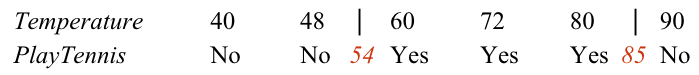
\includegraphics[width=0.5\textwidth]{images/esempio-continuous-valued-attributes.png}
    \end{figure}

    \hspace{-15pt}Determinare le soglie dei candidati calcolando la media dei valori consecutivi dove c'è un cambio di classificazione: (48+60)/2 = 54 e (80/90)/2 = 85.\\
    Valutare le soglie dei candidati (attributi) in base a guadagno di informazioni. La temperatura migliore è $\>$ 54. Quindi, il nuovo attributo compete con gli altri.
\end{example}

\subsubsection{Gestire dati di training incompleti}
Come possiamo affrontare il problema che il valore di alcuni attributi potrebbe \textbf{mancare}? Per esempio risultato dell'esame del sangue in un problema di 
diagnosi medica.\\\\
La strategia: usa altri esempi per indovinare l'attributo (entro dati di addrestramento), imputazioni:
\begin{enumerate}
    \item La cosa più comune è quella di assegnare il valore più comunue tra tutti gli esempi di training al nodo o nodi nella stessa classe.
    \item Assegnare una probabilità $p_i$ ad ogni valore $v_i$, in base alle frequenze, ed assegnare valori all'attributo mancante, in base a questa distribuzione di probabilità (aggiungendo più esempi ponderati dalla probabilità, cioè asegnare la frazione $p_i$ dell'esempio a ciascun albero discendete)
    \item Classificare il nuovo esempio allo tesso modo (ponderazione): e viene scelta la classificazione più probabile.
\end{enumerate}

\subsubsection{Gestire attributi con costi differenti}
Gli attributi dell'istanza possono avere un costo associato: lo faremo preferire alberi decisionali che utilizzano attributi a basso costo.
L'ID3 può essere modificato per tenere conto dei costi. Una prima versione di Tan e Schlimmer (1990)
$$\frac{Gain^2(S,A)}{Const(A)}$$
Una seconda versione di Nunez (1988)
$$\frac{2^{Gain(S,A)} - 1}{(Cost(A) + 1)^w} \hspace{10pt}con\hspace{10pt}w \in [0,1]$$
\textbf{Una vista geometrica}. Confini decisionali che possono essere prodotti da un DT: gli alberi decisionali dividono lo spazio di input 
in rettangoli ed etichette paralleli agli assi, ogni rettangolo con una delle classi K (foglie dell'albero).
\begin{figure}[h!]
    \centering
    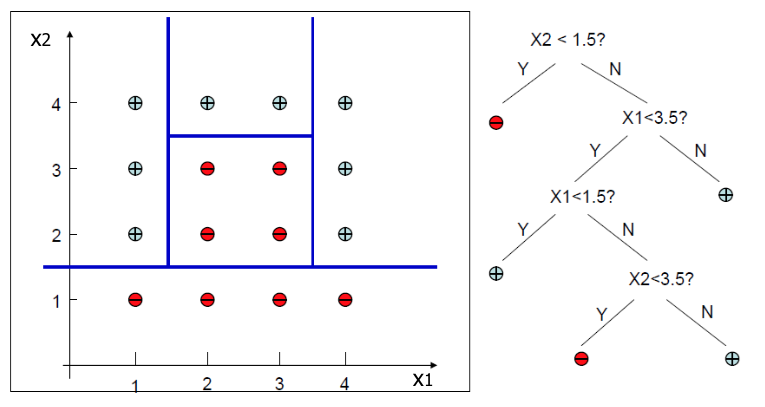
\includegraphics[width=0.6\textwidth]{images/geometry-view-dt.png}
\end{figure}